\documentclass{standalone}
\usepackage{pgfplots}
\pgfplotsset{compat=1.17}

\begin{document}
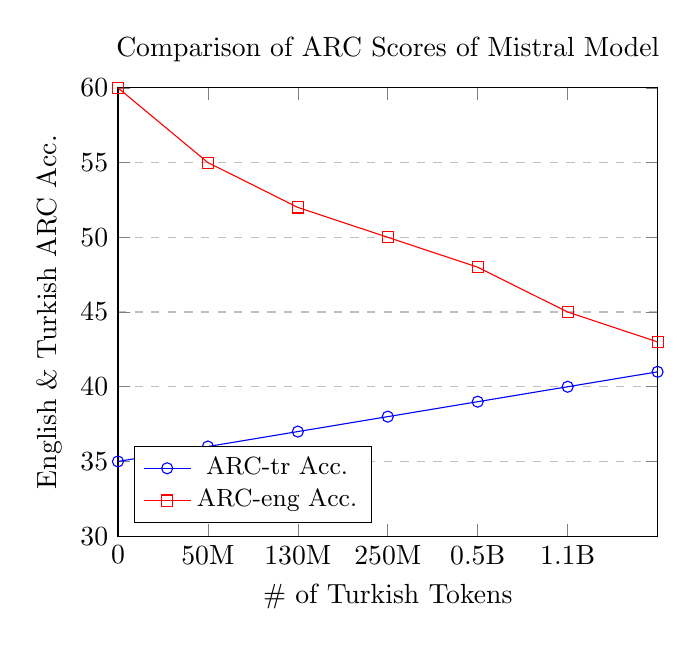
\begin{tikzpicture}
    \begin{axis}[
        title={Comparison of ARC Scores of Mistral Model},
        xlabel={\# of Turkish Tokens},
        ylabel={English \& Turkish ARC Acc.},
        xmin=0, xmax=6,
        ymin=30, ymax=60,
        xtick={0,1,2,3,4,5},
        xticklabels={0, 50M, 130M, 250M, 0.5B, 1.1B, 2.5B},
        ytick={30, 35, 40, 45, 50, 55, 60},
        legend pos=south west,
        ymajorgrids=true,
        grid style=dashed,
        legend style={font=\small},
    ]
    
    % ARC-tr Acc.
    \addplot[
        color=blue,
        mark=o,
        ]
        coordinates {
        (0,35) (1,36) (2,37) (3,38) (4,39) (5,40) (6,41)
        };
    \addlegendentry{ARC-tr Acc.}

    % ARC-eng Acc.
    \addplot[
        color=red,
        mark=square,
        ]
        coordinates {
        (0,60) (1,55) (2,52) (3,50) (4,48) (5,45) (6,43)
        };
    \addlegendentry{ARC-eng Acc.}

    \end{axis}
\end{tikzpicture}
\end{document}